\documentclass[tikz,border=10pt]{standalone}
\usetikzlibrary{calc}

\begin{document}

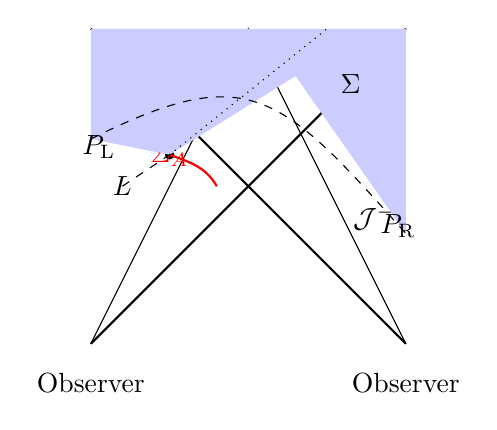
\begin{tikzpicture}[scale=2]
    % Define coordinates for the corners of the diagram
    \coordinate (Jplus) at (0,1);
    \coordinate (Jminus) at (0,0);
    \coordinate (O1) at (-1,-1);
    \coordinate (O2) at (1,-1);

    % Draw the future and past null infinities and the observer positions
    \draw (O1) -- (Jplus) -- (O2);
    \draw (O1) -- (Jminus) -- (O2);
    \node at ($(O1)!0.5!(-1,-1.5)$) {Observer};
    \node at ($(O2)!0.5!(1,-1.5)$) {Observer};

    % Draw the cosmological horizons H_L and H_R
    \draw[black,thick] (-1,1) -- (1,-1);
    \draw[black,thick] (1,1) -- (-1,-1);
    \node at ($(1,0.3)!0.5!(0.3,1)$) {$H_{\rm R}$};
    \node at ($(-1,0.3)!0.5!(-0.3,1)$) {$H_{\rm L}$};
    \node at (0.8,0.8) {$\mathcal{J}^+$};
    \node at (0.8,-0.2) {$\mathcal{J}^-$};

    % Define points for the observers' trajectories and the sphere
    \coordinate (A) at (-0.5,0.2);
    \coordinate (SigmaA) at ($(-0.5,0.2)!0.4!(-0.4,0)$); % point on the static patch boundary
    \coordinate (Sigma) at (0.3,0.7); % arbitrary global spacelike slice
    \coordinate (L) at ($(-0.5,0.2)!0.3!(-0.8,0)$); % part of the trajectory

    % Draw the sphere A as a black dot
    \fill[black] (A) circle (0.03);
    \node[red] at (A) {$\Sigma_A$};

    % Draw the static patch P_L and P_R
    \fill[blue!20] (-1,1) -- (-1,0.3) -- (A) -- (Sigma) -- (0.3,0.7) -- (1,-0.3) -- (1,1) -- cycle;
    \node at ($(-1,0.4)!0.5!(-0.9,0.1)$) {$P_{\rm L}$};
    \node at ($(1,-0.4)!0.5!(0.9,-0.1)$) {$P_{\rm R}$};

    % Draw the observer's trajectory (red curve)
    \draw[red,thick] (-0.5,0.2) to[out=-20,in=120] (-0.2,0);

    % Draw the global spacelike slice (dashed line)
    \draw[dashed] (-1,0.3) .. controls (0,0.8) and (0.2,0.6) .. (1,-0.3);
    \node at ($(1,0.3)!0.5!(0.3,1)$) {$\Sigma$};

    % Draw the arbitrary spacelike slice (black dashed line)
    \draw[black,dashed] (-0.8,0) -- (A);
    \node at (-0.8,0) {$L$};

    % Draw the future lightsheet from A (dotted line)
    \draw[dotted] (A) -- ($(-0.5,0.2)!2!(0,0.6)$); % extend the lightsheet for visualization
\end{tikzpicture}

\end{document}